% Auto-generated figure snippets for main.tex

\begin{figure}[htbp]
\centering
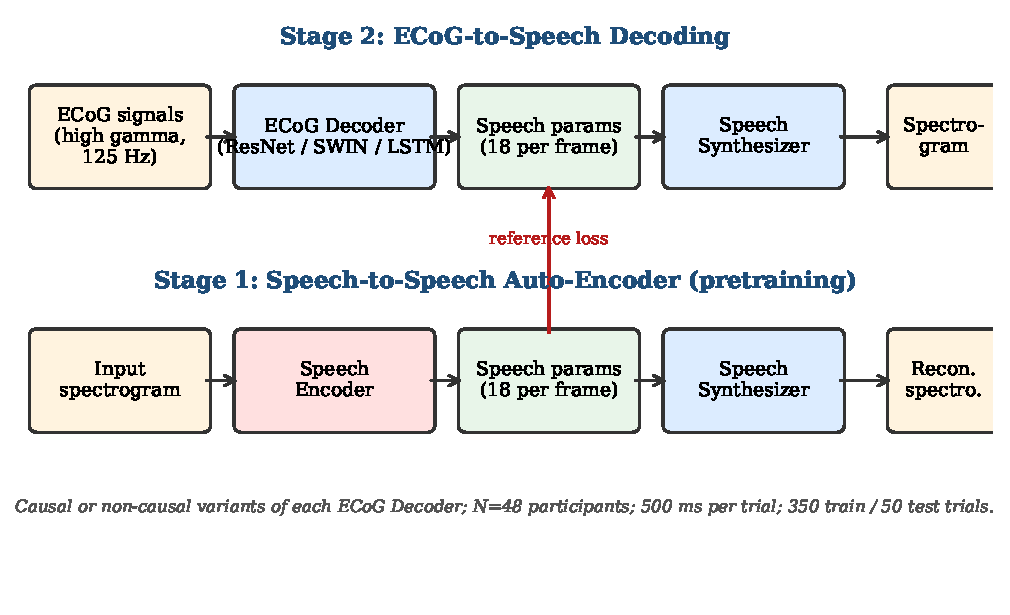
\includegraphics[width=0.7\textwidth]{figures/fig_architecture.pdf}
\caption{Overview of the two-stage neural speech decoding framework.
Stage 1 (bottom) pre-trains a speech-to-speech auto-encoder consisting of a
Speech Encoder and a fully differentiable Speech Synthesizer on the
participant's speech only, producing reference values for 18 interpretable
speech parameters per frame. Stage 2 (top) trains an ECoG Decoder (3D ResNet,
3D Swin Transformer, or LSTM; causal or non-causal) to predict those speech
parameters from ECoG high-gamma activity sampled at 125~Hz. The same
Speech Synthesizer is reused to map the decoded parameters back to a
spectrogram, enabling end-to-end back-propagation of spectral loss. The
reference speech parameters from stage 1 supervise stage 2 through a
reference-parameter loss.}
\label{fig:architecture}
\end{figure}

\begin{figure}[htbp]
\centering
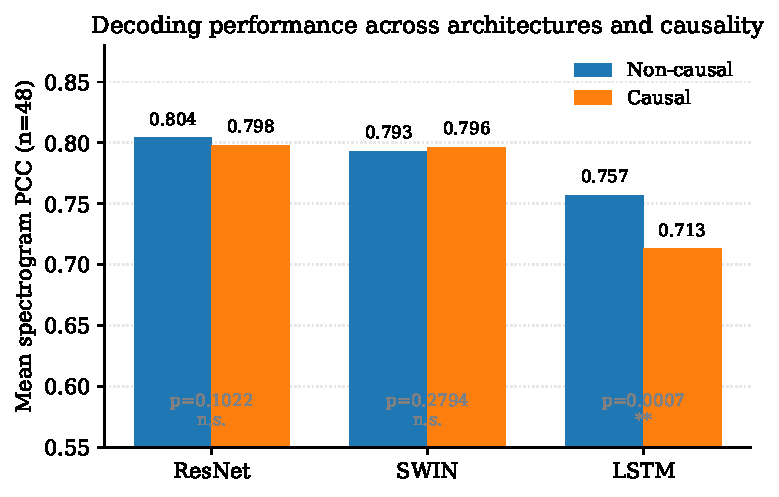
\includegraphics[width=0.72\textwidth]{figures/fig_pcc_models.pdf}
\caption{Mean spectrogram Pearson correlation coefficient (PCC) across
$N=48$ participants for 3D ResNet, 3D Swin Transformer, and LSTM backbones,
evaluated in both non-causal and causal configurations. ResNet achieves the
highest PCC (non-causal $0.804$, causal $0.798$), closely followed by SWIN
($0.793$ and $0.796$). LSTM trails both (non-causal $0.757$, causal
$0.713$). Wilcoxon signed-rank tests comparing the causal and non-causal
variants give $p=0.1022$ for ResNet, $p=0.2794$ for SWIN, and $p=0.0007$ for
LSTM. Only LSTM shows a significant causal/non-causal gap.}
\label{fig:pcc_models}
\end{figure}

\begin{figure}[htbp]
\centering
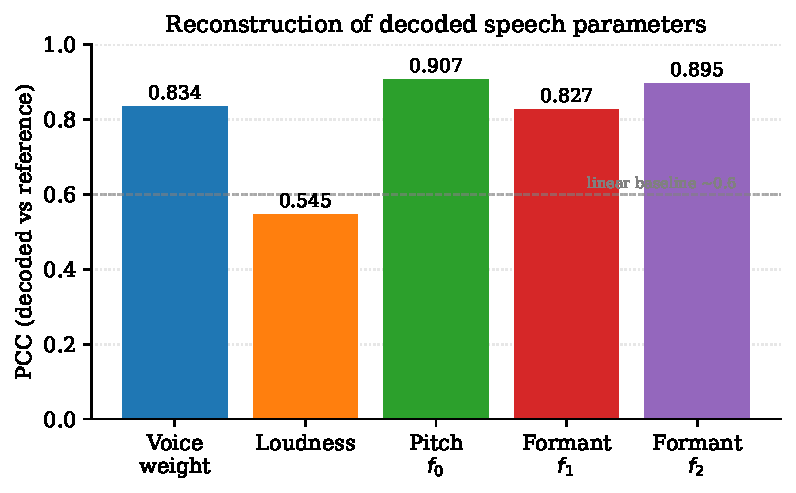
\includegraphics[width=0.72\textwidth]{figures/fig_params.pdf}
\caption{Reconstruction of decoded speech parameters using the causal ResNet
decoder. Mean Pearson correlation between decoded and reference time series
across participants: voice weight $0.834$, loudness $0.545$, pitch $f_0$
$0.907$, first formant $f_1$ $0.827$, second formant $f_2$ $0.895$.
Pitch, voice weight, and the first two formants -- the parameters most
important for intelligibility and participant-specific voice quality -- are
recovered most accurately.}
\label{fig:params}
\end{figure}

\begin{figure}[htbp]
\centering
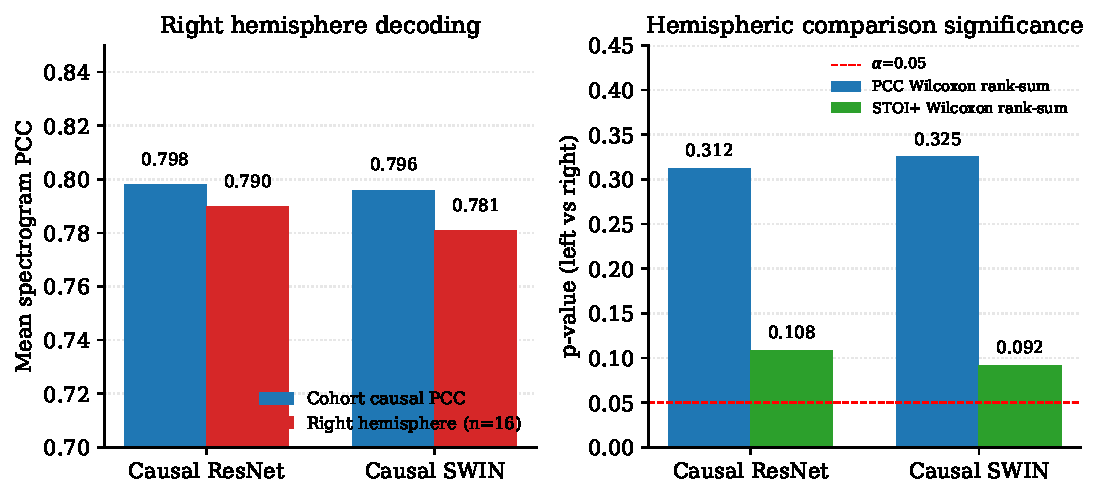
\includegraphics[width=0.95\textwidth]{figures/fig_hemisphere.pdf}
\caption{Right hemisphere decoding. Left: mean spectrogram PCC for causal
ResNet and causal Swin models across the full cohort (causal means $0.798$
and $0.796$ across $n=48$ participants) compared with the right-hemisphere
subset ($n=16$), which reaches PCC $0.790$ (ResNet) and $0.781$ (Swin).
Right: Wilcoxon rank-sum $p$-values for the left-vs-right comparison. PCC
p-values are $0.312$ (ResNet) and $0.325$ (Swin); STOI+ p-values are
$0.108$ (ResNet) and $0.092$ (Swin). None cross the $\alpha=0.05$ threshold
(dashed red line), consistent with the absence of significant hemispheric
differences.}
\label{fig:hemisphere}
\end{figure}
